\chapter{Methodology}
\label{chapter:methodology}

\section{Architecture Overview}
\label{section:architecture_overview}

In this section, I propose a new model for single-concept open-ended visual question answering tasks. The proposed model comprises six main components, as shown in \figureautorefname{ \ref{fig:model_overview}} and outlined briefly below. In the following subsections, I explain the motivations behind each architecture component, along with detailed descriptions of their composition. I refer the reader to the \nomref{frontmatter:nomenclature} in the front matter for descriptions of common nomenclature used in this chapter.


\begin{figure}[htbp]
    \centering
    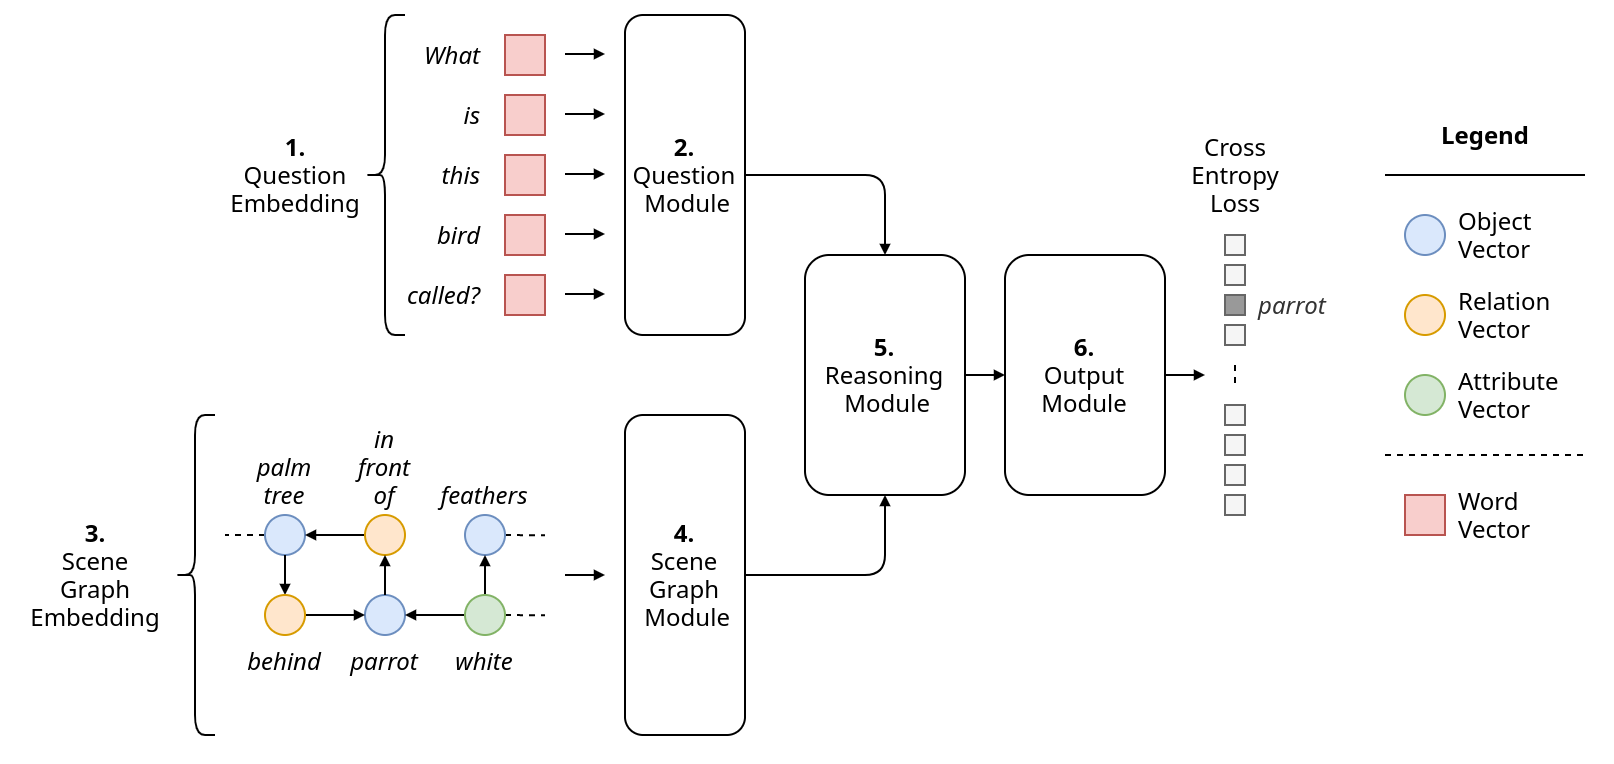
\includegraphics[width=\textwidth]{model_overview.png}
    \caption[An overview of the proposed visual-question-answering model.]{\textbf{Model Overview.} A high-level overview of the proposed visual-question-answering model. Both questions and scene graphs are embedded as tensors, then contextual features are obtained by the question and scene graph modules. Finally, the reasoning and output modules formulate an answer to the question.}
    \label{fig:model_overview}
\end{figure}

\textbf{Question embedding:} In classic NLP fashion, the question embedding component is responsible for the preprocessing and vectorisation of raw question data for use by the rest of the model.

\textbf{Question module:} The question module has two main roles: the first is to learn a sequence of word embeddings that capture the relevant features of each question word in the context of the question as a whole. Secondly, the question module learns a question-level embedding that contains information about the question as a whole.

\textbf{Scene graph embedding:} The scene graph embedding model is responsible for the preprocessing and vectorisation of scene graph data. In this dissertation, I use ground-truth scene graphs from the GQA dataset to evaluate the effectiveness of various scene graph modules under perfect-sight conditions. This component can be readily extended to utilise the output of existing scene graph generation models \cite{yang2018graph, li2019relation}, yielding a true end-to-end VQA model.

\textbf{Scene graph module:} The primary goal of the scene graph module is to learn a dense representation of scene graph features that can be used as a knowledge-base for the reasoning module to draw information from when answering questions.

\textbf{Reasoning module:} Given the output features of the scene graph and question modules, the reasoning module is in charge of determining which visual features are relevant to the question and vice-versa. The reasoning capabilities of many existing VQA models could be leveraged here; I justify my reasoning module of choice and describe its implementation in detail in \sectionautorefname{ \ref{section:reasoning_module}}.

\textbf{Output module:} The output module is the simplest part of the architecture, and is responsible for transforming the output of the reasoning module into a concrete answer to the input question. I delve into the design decisions behind the output module and how it might be modified for other VQA tasks in \sectionautorefname{ \ref{section:output_module}}.

\section{Question Embedding and Module}
\label{section:question_embedding_and_module}

\subsubsection{Preprocessing and Embedding}

The question embedding component of the architecture is responsible for two major tasks: preprocessing and vectorisation. The preprocessing step is performed prior to the training of the model, where vectorisation of preprocessed question words occurs at runtime. 

I use a neural preprocessing pipeline for each raw question string in the dataset, comprising tokenisation, part-of-speech (POS) tagging, lemmatisation and dependency parsing steps.\footnote{For this architecture, only the tokenisation step is required since the question module uses word embeddings but not syntactic dependency information. Graph-based question modules use syntactic dependencies for graph construction, as described in \subsectionautorefname{ \ref{subsec:question_module_ablations}}.} For reproducibility, I use the Stanza NLP package \cite{qi2020stanza} for all steps of the pipeline.

After tokenisation, each question \(q\) is represented as a sequence of tokens \((t_1, ..., t_{l_q})\), where \(l_q\) is the number of tokens in the question. For each question \(q\), each  token \(t\) is converted to an index to enable vector embedding lookups during training. A mapping of all question tokens to their respective indices is kept, with indices being shared between the training and validation sets. Reference answers are converted to indices in a similar fashion, however they are not tokenised first: multi-word answers like \textit{parking meter} or \textit{cutting board} are treated as a single concept, identically to single-word answers like \textit{bed}. This ensures  multi-word answers can be predicted just as easily as single-word answers and allows the output module to treat the question-answering task as a multi-class classification problem across the set of all candidate answers.

At runtime, each question token is converted to a \(d_{H_q} = 300\) dimensional GloVe vector \cite{pennington2014glove}, then token embeddings for a given question are stacked together, yielding a matrix of question features \(H_q \in \R^{l_q \times d_{H_q}}\) where \(l_q\) is the number of tokens in the question. For a batch of questions \(Q_{[i:i+k]}\) the corresponding features \(\{H_{q_i}, ..., H_{q_{i+k-1}}\}\) are padded with zeros along the first dimension and then stacked to yield a batch of question features \(H_{Q_{[i:i+k]}} \in \R^{k \times l \times d_{H_q}}\), where \(l = \max_{i \leq j < i+k} l_{q_j}\), the number of tokens in the longest question in the batch.\footnote{In practice, \(H_{Q_{[i:i+k]}}\) is constructed and batched similarly to \(H_{R_{[i:i+k]}}\) as described in \subsectionautorefname{ \ref{sec:scene_graph_embedding_details}} to allow the training of graph-based question modules. I avoid graph-specific notation here for clarity, reserving it for \subsectionautorefname{ \ref{subsec:question_module_ablations}}, where I discuss graph-based question module variants in depth.}

\subsubsection{Question Module}

Given a batch of question features \(H_{Q_{[i:i+k]}}\) from the question embedding component, the question module is responsible for learning a holistic representation of each question in the batch, as well as capturing the syntactic and contextual dependencies between words in each question. More formally, the question module learns a  \(d_{K_q}\) dimensional vector for each of the \(k\) questions in the batch, denoted \(\mathcal{Q}_{Q_{[i:i+k]}} \in \R^{k \times d_{K_q}}\), as well as a knowledge base of contextual question words \(K_{Q_{[i:i+k]}} \in \R^{k \times l \times d_{K_q}}\).

A variety of architectures have been used to obtain these representations in VQA contexts, the most common being recurrent models like LSTMs \cite{hochreiter1997long} or GRUs \cite{cho2014learning}, used by \cite{perez2017film, hudson2018compositional, lu2016hierarchical, yu2019deep} and \cite{anderson2018bottom, teney2018tips, li2019relation, liu2019densely, gao2019dynamic, kim2018bilinear} respectively. More recently, others have explored graph-based question processing architectures like GCNs and GATs for text classification \cite{yao2019graph, liu2020tensor} and now VQA \cite{huang2020aligned}. After trying a variety of question modules, my initial experiments showed more promising results with a traditional bidirectional LSTM, depicted in \figureautorefname{ \ref{fig:question_module_bilstm}}. I compare and analyse the performance of various question modules in \subsectionautorefname{ \ref{subsec:question_module_ablations}}.

\begin{figure}[htbp]
    \centering
    \begin{subfigure}[l]{0.4\textwidth}
    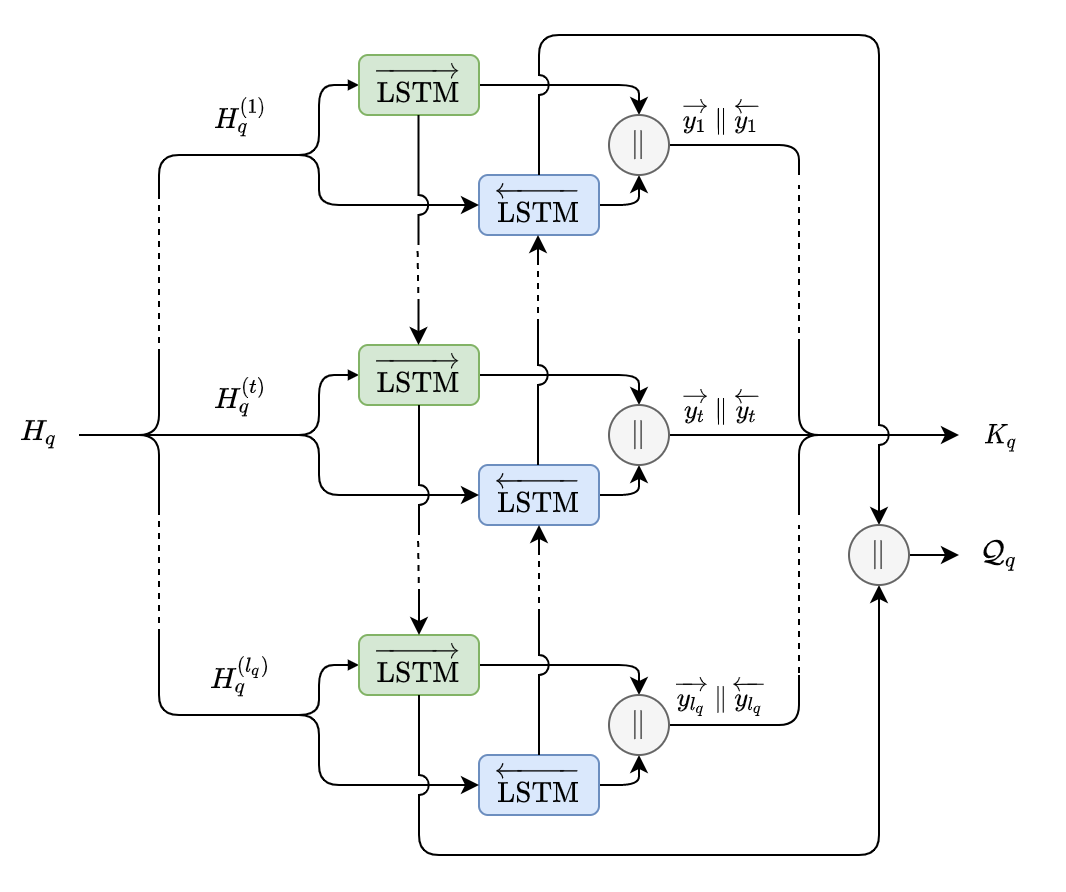
\includegraphics[width=\textwidth]{bilstm.png}
    \end{subfigure}
    \begin{subfigure}[r]{0.59\textwidth}
        \begin{equation}
            \overrightarrow{y_t} = \overrightarrow{\text{LSTM}}(H_q^{(t)}) \in \R^\frac{d_{K_q}}{2}, 1 \leq t \leq l_q\\
            \label{equation:question_module_forward_y_t}
        \end{equation}
        \begin{equation}
            \overleftarrow{y_t} = \overleftarrow{\text{LSTM}}(H_q^{(t)}) \in \R^\frac{d_{K_q}}{2}, 1 \leq t \leq l_q\\
            \label{equation:question_module_backward_y_t}
        \end{equation}
        \begin{equation}
            K_q = \left [ \overrightarrow{y_0} \cat \overleftarrow{y_0}, ..., \overrightarrow{y_{l_q}} \cat \overleftarrow{y_{l_q}}\right] \in \R^{l_q \times d_{K_q}}\\
            \label{equation:question_module_K_q}
        \end{equation}
        \begin{equation}
            \mathcal{Q}_q = \overrightarrow{h_{l_q}}\cat \overleftarrow{h_{1}} \in \R^{d_{K_q}}
            \label{equation:question_module_Q_q}
        \end{equation}
    \end{subfigure}
    \caption[An overview of the question module architecture.]{\textbf{Question module architecture.} For each question \(q\), the question module takes a matrix of question embeddings \(H_q\) as an input, and produces a knowledge-base of contextual word information \(K_q\) as well as a question embedding vector \(\mathcal{Q}_q\).}
    \label{fig:question_module_bilstm}
\end{figure}

To obtain \(K_{Q_{[i:i+k]}}\) and \(\mathcal{Q}_{Q_{[i:i+k]}}\), batched question embeddings \(H_{Q_{[i:i+k]}}\) are passed through a single-layer bidirectional LSTM, with each direction having a hidden layer dimension of \(\frac{d_{K_q}}{2} = 128\). I refer the reader to \sectionautorefname{ \ref{sec:hyperparameter_optimisation}} for details on how these parameters were determined. For each question \(q \in Q_{[i:i+k]}\), the contextual knowledge-base vectors for each word are the concatenated outputs of the forward and backward LSTMs \(\overrightarrow{y_t}\) and \(\overleftarrow{y_t}\) at each time step \(t\) respectively. In \equationautorefname{ \ref{equation:question_module_forward_y_t}} and \equationautorefname{ \ref{equation:question_module_backward_y_t}}, I represent the \(t\)th word in \(q\) as \(H_q^{(t)}\), which is used to derive \(\overrightarrow{y_t}\) and \(\overleftarrow{y_t}\) for each \(t\). Since LSTM weights are shared between time steps, the \(t\)th step of the forward LSTM is able to capture contextual information from the previous \(t-1\) steps, provided \(t\) is not excessively large.\footnote{In the GQA and CLEVR datasets, the longest questions are in the order of 25-30 words.} The same can be said for the backward LSTM, except it captures contextual information starting from the end of the question, as shown in \figureautorefname{ \ref{fig:question_module_bilstm}}. After obtaining \(\overrightarrow{y_t}\) and \(\overleftarrow{y_t}\) for each \(1 \leq t \leq l_q\), the contextual knowledge-base \(K_q\) is built according to \equationautorefname{ \ref{equation:question_module_K_q}}. Similarly to \cite{hudson2018compositional}, the holistic representation \(\mathcal{Q}_q\) of a question \(q\) is obtained by concatenating the final hidden states of the forward and backward LSTM passes, since they contain contextual information for all question words in each direction. More formally, the respective forward and backward final hidden states \(\overrightarrow{h_{l_q}}\) and \(\overleftarrow{h_{1}}\) are combined according to \equationautorefname{ \ref{equation:question_module_Q_q}} to yield \(\mathcal{Q}_q\).

 Of course, all questions in the batch are processed simultaneously to yield the entire contextual knowledge base \(K_{Q_{[i:i+k]}} = [K_{q_i}, ..., K_{q_{i+k-1}}]\) and question representations \(\mathcal{Q}_{Q_{[i:i+k]}} = [\mathcal{Q}_{q_i}, ..., \mathcal{Q}_{q_{i+k-1}}]\). Both \(K_{Q_{[i:i+k]}}\) and \(\mathcal{Q}_{Q_{[i:i+k]}}\) are inputs to the reasoning module, as described in \sectionautorefname{ \ref{section:reasoning_module}}.

\section{Scene Graph Embedding and Module}
\label{section:scene_graph_embedding}

\subsection{Motivation}
\label{section:scene_graph_embedding_motivation}

The primary goal of the scene graph embedding process is to build a directed graph \(\mathcal{G}_r = (\mathcal{V}_r, \mathcal{E}_r)\) and an associated node feature matrix \(H_r \in \R^{n_r \times d_{H_r}}\) from a visual representation \(r\). These node features are essential information for the scene graph module, a three-layer Graph Attention Network (GAT) \cite{velivckovic2017graph} which utilises node-based graph convolutions to capture dependencies and relationships between nodes in the graph. In this dissertation, I intentionally use gold-standard scene graphs as a visual input to evaluate the effectiveness of different scene graph modules, as discussed in \sectionautorefname{ \ref{sec:ablation_studies}}. Since my primary focus is on scene graphs as a visual input signal, I will consider all general visual representations \(r\) to be scene graphs for the remainder of this section.

Both the GQA and CLEVR datasets contain ground-truth scene graph information for each image in the training and validation sets. Although different datasets store scene graph information differently, the three basic components of a scene graph are objects, relationships and attributes. For example, the CLEVR dataset contains three object types (cube, sphere, cylinder), twelve attribute types covering size (small, large), material (metal, rubber) and colour (red, green, blue, yellow, purple, cyan, brown, grey), and four spatial relationships (left, right, in front, behind). The GQA dataset is more complex, containing, a total of 1703 unique objects, 310 unique relations, and 617 unique attributes across the combined train and validation sets. Adopting common notation from \cite{hudson2019gqa, li2019relation, yang2018graph}, each directed relationship between two objects in a scene graph can be described as a triplet \texttt{<subject, relation, object>}, \textit{e.g.} \texttt{<parrot, behind, fence>}\footnote{Although the \texttt{subject} and \texttt{object} are both represented by objects in a scene graph, this notation disambiguates the direction of the relationship by drawing upon well-defined grammatical terms, \textit{e.g.} \texttt{<parrot, behind, fence>} corresponds to the clause: \textit{The parrot is behind the fence}.}. For scene graphs containing attributes, we can use a pair \texttt{<object, attribute>} to denote attribute associations, \textit{e.g.} \texttt{<parrot, white>}. More formally, we can represent a raw scene graph 
\(r\) like so:

\begin{align*}
    r \quad & \text{A scene graph, } (r_o, r_r, r_a, r_{(s,r,o)}, r_{(o, a)})\\
    r_o \quad  & \text{The sequence of all objects in \(r\), not necessarily unique.}\\
    r_r \quad & \text{The set of all unique relations in \(r\)}\\
    r_a \quad & \text{The set of all unique attributes in \(r\)}\\
    r_{(s,r,o)} \quad & \text{The sequence of (subject, relation, object) triples in } r,\\
    & ((x, y, z) \mid x \in r_o, y \in r_r, z \in r_o)\\
    r_{(o, a)} \quad & \text{The sequence of (object, attribute) pairs in \(r\),}\\
    & ((x, y) \mid x \in r_o, y \in r_a)\\
\end{align*}

Note that I represent \(r_o\) as a sequence and not a set since some scene graphs \(r\) may contain multiple instances of the same type of object, \textit{e.g.} an image of a city sidewalk may contain multiple people, each of which have their own attributes and relationships with other objects in the scene.

There are multiple points to consider when converting a general scene graph representation \(r\) to its directed graph \(\mathcal{G}_r\) and associated node features \(H_r\); my scene graph embedding choice has two main motivations:

\begin{enumerate}
    \item The scene graph embedding needs to provide adequate information to answer a variety of questions, regardless of whether they ask about an object \textit{e.g. What type of bird is that?}, an attribute \textit{e.g. What colour is the bird?} or a relationship between two objects \textit{e.g. Is the bird behind the fence?}.
    \item The goal of the scene graph module is to update the initial object, attribute and relation embeddings created by the scene graph embedding stage to include dependency information. These dependencies are readily captured by existing node-based graph convolutions, however, to utilise these methods, all features that may be relevant to question answering must be represented as node features.
\end{enumerate}

The first point insinuates that objects, attributes and relations should be embedded similarly in the scene graph to aid the reasoning module in its decisions; if we embedded objects differently to relations in the scene graph, then the reasoning module has to learn to respond differently to questions that ask about objects versus those that ask about relationships between objects. Conversely, by embedding relationships, attributes and objects in a similar manner, I hypothesise that the reasoning module is more likely to transfer reasoning skills between similarly-posed but differently-targeted questions.

The second motivation poses an issue: assume we have \(n_o\) objects and \(n_r\) relations for any particular scene graph. Assuming all \(n_o\) objects are represented as nodes in the graph, then embedding every relationship between two objects as a node instead of an edge increases the upper bound of nodes in the graph from \(O(n_o)\) to \(O(n_o + n_r) = O(n_o^2)\) nodes, increasing the computational complexity of any parts of the model that operate on the graph's nodes. Conversely, omitting relational data from node embeddings may hinder the model's ability to answer questions requiring logical reasoning about relationships between objects. I explore this trade-off between computational complexity and performance in \sectionautorefname{ \ref{sec:ablation_studies}}.

{\color{red} TODO: Consider number of edges due to relations increases from \(n_r \rightarrow 2n_r\). Since GAT/GCN complexity is bounded by number of edges, this is acceptable, under the condition that we can handle sparse operations efficiently, since all relation nodes only ever have one incoming and one outgoing edge.}

\subsection{Technical details}
\label{sec:scene_graph_embedding_details}

\subsubsection{Preprocessing and Embedding}
The preprocessing of objects, relations and attributes is similar to the way answers were processed in the question embedding embedding step; each unique object, attribute or relation is converted to a unique index regardless of whether it is a single-word concept like \textit{parrot} or a multi-word concept like \textit{to the left of}. To simplify graph construction and embedding lookups, I use a combined index set for objects, relations and attributes, computed across the combined train and validation sets \(S\). All unique objects, relations and attributes are converted to indices, with objects, relations and attributes corresponding to indices in the ranges \([0, |S_o|)\), \([|S_o|, |S_o| + |S_r|)\) and  \([|S_o| + |S_r|, |S_o| + |S_r| + |S_a|)\) respectively, where \(S_o = \bigcup_{r \in R} \{x \mid x \in r_o\}\) is the set of unique scene graph objects in \(S\), \(S_r = \bigcup_{r \in R} r_r\) is the set of unique scene graph relations in \(S\) and \(S_a = \bigcup_{r \in R} r_a\) is the set of unique scene graph  attributes in \(S\). By computing the sets of unique objects, attributes and relations separately, I ensure that words which may be used as an object or an attribute \textit{e.g. glass} are given an two indices, one in the object index subset and one in the attribute index subset. Consequently, the scene graph module is able to learn different embeddings for the same word based on the contexts in which they occur in a scene graph.

At runtime, each object, relation and attribute index is associated with a \(d_{H_r} = 300\) dimensional GloVe vector. For multi-word objects, relations and attributes, I average the GloVe embeddings for each word to avoid out-of-vocabulary (OOV) issues. All vectors are then stacked together to produce an embedding matrix of scene graph node features \(H_S\) spanning the object, relation and attribute vocabulary of the combined train and validation datasets \(S\), \textit{i.e.} \(H_S \in \R^{(|S_o| + |S_r| + |S_a|) \times d_{H_r}}\). The first \(|S_o|\) rows correspond to object embeddings, the next \(|S_r|\) to relations, and the last \(|S_a|\) to attributes. These global node features \(H_S\) are shared by all scene graphs, and fine-tuned via backpropagation  during training. This fine-tuning is particularly important for multi-word relations like \textit{to the right of} and \textit{to the left of}, where the averaged GloVe vectors of individual words may not capture the meaning of the relation effectively.

Given a single preprocessed scene graph \(r\), the elements of \(r_o, r_r\) and \(r_a\) are all represented as indices, with each index corresponding to a row in \(H_S\). Obtaining the relevant embeddings for a scene graph \(r\) is thus as simple as selecting all rows in \(H_S\) indexed by a elements in \(\{x \mid x \in r_o\}, r_r\) and \(r_a\), the sets of unique object, relation and attribute indices respectively. This yields a node feature matrix \(H_r \in \R^{n_r \times d_{H_r}}\), where \(n_r = |\{x \mid x \in r_o\}| + |r_r| + |r_a|\). The same applies for a batch of scene graphs \(R_{[i:i+k]}\), except unique indices are computed across all objects, relations and attributes in the batch to yield a node feature matrix
\(H_{R_{[i:i+k]}} \in \R^{n_{R_{[i:i+k]}} \times d_{H_r}}\), where \(n_{R_{[i:i+k]}} = |\cup_{r \in R_{[i:i+k]}}\{x \mid x \in r_o\}| + |\cup_{r \in R_{[i:i+k]}}r_r| + |\cup_{r \in R_{[i:i+k]}}r_a|\).

After retrieving relevant node embeddings, the final directed graph \(\mathcal{G}_r\) is created according to \algorithmcfname{ \ref{algorithm:scene_graph_construction}}. Since each vertex in the graph corresponds to either an object, relation or attribute index, the embedding for that vertex is easily obtained from the node feature matrix \(H_r\).

\begin{algorithm}[htbp]
    \Function{\(r_o, r_r, r_a, r_{(s, r, o)}, r_{(o, a)}\)}{
        \(\mathcal{V}_\text{obj}, \mathcal{V}_\text{rel}, \mathcal{V}_\text{attr} \leftarrow \emptyset, \emptyset, \emptyset\)\\
        \(\mathcal{E}_{\text{(obj,rel)}}, \mathcal{E}_{\text{(rel,obj)}},
        \mathcal{E}_{\text{(obj,obj)}},
        \mathcal{E}_{\text{(attr,obj)}} \leftarrow \emptyset, \emptyset, \emptyset, \emptyset\)\\
        \ForEach{\(x \in r_o\)}{
            Construct a vertex \(v_x\) corresponding to object index \(x\)\\
            \(\mathcal{V}_\text{obj} \leftarrow \mathcal{V}_\text{obj} \cup \{v_x\}\)\\
        }
        \ForEach{\((x, y, z) \in r_{(s, r, o)}\)}{
            Construct a vertex \(v_y\) corresponding to relation index \(y\)\\
            \(\mathcal{V}_\text{rel} \leftarrow \mathcal{V}_\text{rel} \cup \{v_y\}\)\\
            Look up vertices \(v_x, v_z\)in \(\mathcal{V}_\text{obj}\) corresponding to indices \(x\) and \(y\) respectively.\\
            \(\mathcal{E}_{\text{(obj,rel)}} \leftarrow \mathcal{E}_{\text{(obj,rel)}} \cup \{(v_x, v_y)\}\)\\
            \(\mathcal{E}_{\text{(rel,obj)}} \leftarrow \mathcal{E}_{\text{(rel,obj)}} \cup \{(v_y, v_z)\}\)\\
            \(\mathcal{E}_{\text{(obj,obj)}} \leftarrow \mathcal{E}_{\text{(obj,obj)}} \cup \{(v_x, v_z)\}\)\\
        }
        \ForEach{\(x \in r_a\)}{
            Construct a vertex \(v_x\) corresponding to attribute index \(x\)\\
            \(\mathcal{V}_\text{attr} \leftarrow \mathcal{V}_\text{attr} \cup \{v_x\}\)\\
        }
        \ForEach{\((x, y) \in r_{(o, a)}\)}{
            Look up vertex \(v_x \in \mathcal{V}_\text{obj}\) corresponding to object index \(x\).\\
            Look up vertex \(v_y \in \mathcal{V}_\text{attr}\) corresponding to attribute index \(y\).\\
            \(\mathcal{E}_{\text{(attr,obj)}} \leftarrow \mathcal{E}_{\text{(attr,obj)}} \cup \{(v_y, v_x)\}\)
        }
        \(\mathcal{V}_r \leftarrow \mathcal{V}_\text{obj} \sqcup \mathcal{V}_\text{rel} \sqcup \mathcal{V}_\text{attr}\)\\
        \(\mathcal{E}_r \leftarrow \mathcal{E}_{\text{(obj,rel)}} \sqcup \mathcal{E}_{\text{(rel,obj)}} \sqcup
        \mathcal{E}_{\text{(obj,obj)}} \sqcup
        \mathcal{E}_{\text{(attr,obj)}}\)\\
        \Return \((\mathcal{V}_r, \mathcal{E}_r)\)
    }
    \caption[Scene Graph Construction Algorithm]{Scene Graph Construction Algorithm}
    \label{algorithm:scene_graph_construction}
\end{algorithm}

\begin{figure}[htbp]
    \centering
    \begin{subfigure}[l]{0.49\textwidth}
        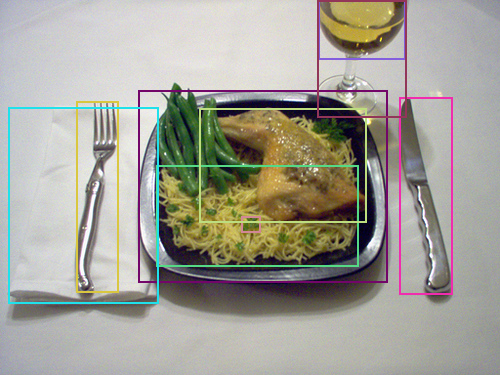
\includegraphics[width=\textwidth]{scene_graph_construction_image.png}
        \label{fig:scene_graph_construction_image}
    \end{subfigure}
    \begin{subfigure}[r]{0.49\textwidth}
        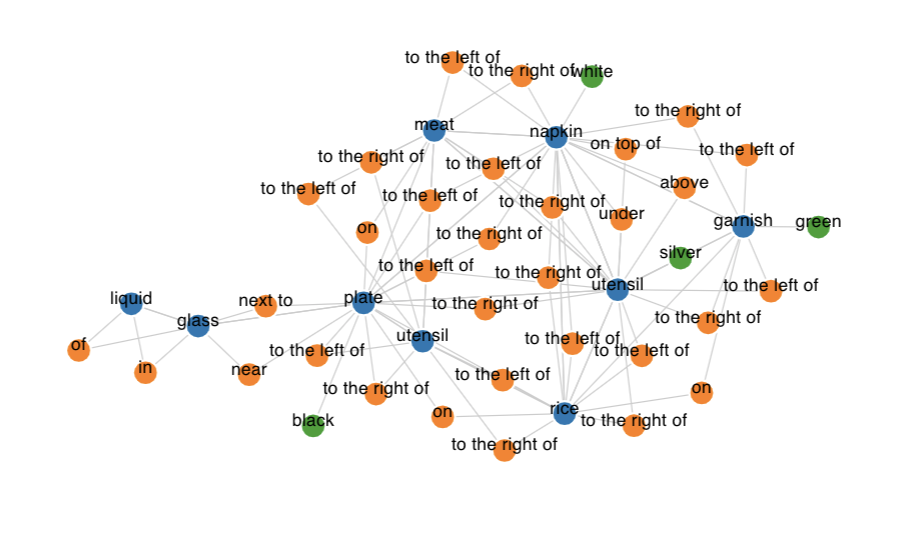
\includegraphics[width=\textwidth]{scene_graph_construction_graph.png}
        \label{fig:scene_graph_construction_graph}
    \end{subfigure}
    \caption[An image from the GQA dataset and its corresponding scene graph \(\mathcal{G}_r\).]{A sample from the GQA validation set and its scene graph \(\mathcal{G}_r\), constructed according to \algorithmcfname{ \ref{algorithm:scene_graph_construction}}. Object, relation and attribute nodes are coloured blue, orange and green respectively.}
    \label{fig:scene_graph_construction}
\end{figure}

For clarity, I represent \(\mathcal{V}_r\) and \(\mathcal{V}_e\) as unions of disjoint subsets in \algorithmcfname{ \ref{algorithm:scene_graph_construction}}, where each subset of vertices and edges is constructed slightly differently. To gain a better understanding of the different types of vertices and edges in \(\mathcal{G}_r\) and the motivations behind their inclusion in the graph, I explore each of these subsets separately, giving some examples from \figureautorefname{ \ref{fig:scene_graph_construction}}.

\(\mathcal{V}_\text{obj}\) contains a node for each object in \(r_o\). Since \(r_o\) is a sequence and not a set, \(\mathcal{V}_v\) may contain multiple nodes corresponding to objects that have the same type/index but refer to different entities in \(r\). We see this in \figureautorefname{ \ref{fig:scene_graph_construction}}, where there are two object nodes labelled \textit{utensil}, one corresponding to a fork and the other to a knife. Moreover, I use the sequence \(r_o\) for object node creation over the objects in \(r_{(s, r, o)}\) or \(r_{(o, a)}\), since \(r_o\) may contain objects with no associated relations or attributes. As a result, \(\mathcal{G}_r\) often contains multiple connected components.

\(\mathcal{V}_\text{rel}\) contains a node for each relation in \(r_{s, r, o}\). Again, since \(r_{s, r, o}\) is a sequence and not a set, \(\mathcal{V}_v\) may contain multiple nodes corresponding to relations with the type/index but with differing source and target entities in \(r\). This is clear in \figureautorefname{ \ref{fig:scene_graph_construction}}, where we see many instances of common relations like \textit{to the left of} and \textit{to the right of}.

\(\mathcal{V}_\text{attr}\) contains a node for each attribute in \(r_a\). Since \(r_a\) is a set, only a single node is created for each type of attribute. The construction of \(\mathcal{E}_\text{attr,obj}\) ensures that attribute nodes can only ever have outgoing edges, meaning their embeddings are never updated by graph convolutions in the scene graph module. As a result, there is no need to create multiple nodes for attributes with the same name/index but different target objects.

\(\mathcal{E}_{\text{(obj,rel)}}\) only contains edges from objects to relations (blue to orange in \figureautorefname{ \ref{fig:scene_graph_construction}}), allowing the scene graph module to capture subject-relation interactions. Conversely, \(\mathcal{E}_{\text{(rel,obj)}}\) contains edges from relations to objects (orange to blue), allowing the scene graph module to learn object representations that include information about incoming relations, as well as the subject of those relations via second-order message passing. \(\mathcal{E}_{\text{(obj,obj)}}\) contains edges from objects to objects (blue to blue) whenever there is a relation between the two objects. This allows direct message passing between object nodes, which may prove useful in cases where we care less about relationship type and more about whether two objects are related or not \textit{e.g.} for logical or counting-based questions. Lastly, \(\mathcal{E}_{\text{(attr,obj)}}\) \(\mathcal{E}_r\) contains an edge from each attribute to its associated object (green to blue). These edges encourage the fortification of object representations with attribute information, allowing objects of the same type to be distinguished according to their individual features.

\subsubsection{Scene Graph Module}
{\color{red} TODO: Consider moving to introduction or literature review.\\
\color{blue}
Originally proposed for inductive and transductive node-classification tasks, the graph attention network (GAT) \cite{velivckovic2017graph} has gained the attention of computer vision researchers in the last three years, particularly for image-to-scene-graph \cite{yang2018graph} and text-to-scene-graph \cite{han2020victr} generation, and, more recently, visual question answering \cite{li2019relation, huang2020aligned}.
Prior works have demonstrated the effectiveness of attention-based graph convolutions for processing scene graph information in a variety of different contexts, with ReGAT \cite{li2019relation} achieving state-of-the-art results on the VQA 2.0 and VQA-CP v2 datasets in \citeyear{li2019relation}, and DC-GCN \cite{huang2020aligned} achieving comparable or greater performance than ReGAT on various VQA 2.0 subtasks in \citeyear{huang2020aligned}. However, both of these models do not evaluate the effectiveness of GATs for scene graph processing using gold-standard scene graph information. This makes it difficult to determine how much of the reported performance gain over non-scene-graph-based models can be accredited to the GAT architecture, and how much is due to the inclusion of generated scene graph information.}

The primary goal of the scene graph module is to learn a knowledge-base of scene graph features that captures dependencies between scene graph objects, relationships and attributes. More formally, for each batch of scene graphs \(\mathcal{G}_{R_{[i:i+k]}}\) and associated node embeddings \(H_{R_{[i:i+k]}} \in \R^{n_{R_{[i:i+k]}} \times d_{H_r}}\), the scene graph module builds a dependency-aware knowledge-base \(K_{R_{[i:i+k]}} \in \R^{n_{R_{[i:i+k]}} \times d_{K_r}}\)\footnote{For ease of reference, I remind the reader that \(n_{R_{[i:i+k]}} = |\cup_{r \in R_{[i:i+k]}}\{x \mid x \in r_o\}| + |\cup_{r \in R_{[i:i+k]}}r_r| + |\cup_{r \in R_{[i:i+k]}}r_a|\) is the sum of unique object, relation and attribute node indices, computed across a batch of scene graphs \(R_{[i:i+k]}\).}

% Given a graph \(\mathcal{G}_r\) and associated node feature matrix \(H_r\), I use a GAT with three convolutional layers to learn a knowledge-base of scene graph features  \(K_r \in \R^{|\mathcal{V}_r| \times d_{K_r}}\).

Batch: \(R_{[i:i+k]}\)

In order to leverage the computational benefits of sparse tensor operations implemented in PyG \cite{fey2019fast},
{\color{red} TODO: Talk about batching operations}


{\color{red} TODO: Verify this still holds: Interestingly, using non-linearities such as ReLU between GAT convolutions destroys the rich information provided by the GloVe embeddings by setting negative values to zero.}

% CLEVR scene graph example:

% \begin{verbatim}
%     {"image_index": 0, "objects": [{"color": "blue", "size": "large", "rotation": 269.8517172617167, "shape": "cube", "3d_coords": [-1.3705521821975708, 2.0794010162353516, 0.699999988079071], "material": "rubber", "pixel_coords": [269, 88, 12.661545753479004]}, {"color": "green", "size": "large", "rotation": 292.2219458666971, "shape": "cylinder", "3d_coords": [-2.9289753437042236, -1.7488206624984741, 0.699999988079071], "material": "metal", "pixel_coords": [93, 108, 11.522202491760254]}, {"color": "cyan", "size": "small", "rotation": 25.545135239473026, "shape": "cube", "3d_coords": [1.5515961647033691, 0.6776641607284546, 0.3499999940395355], "material": "rubber", "pixel_coords": [319, 162, 10.045343399047852]}, {"color": "brown", "size": "large", "rotation": 327.3489188814305, "shape": "cylinder", "3d_coords": [-0.25301405787467957, -2.3089325428009033, 0.699999988079071], "material": "metal", "pixel_coords": [132, 159, 9.392304420471191]}, {"color": "gray", "size": "small", "rotation": 6.325183772442613, "shape": "cube", "3d_coords": [1.018894076347351, -1.93693208694458, 0.3499999940395355], "material": "rubber", "pixel_coords": [192, 197, 8.907766342163086]}, {"color": "brown", "size": "large", "rotation": 25.96049348342493, "shape": "sphere", "3d_coords": [0.43993687629699707, 2.9987525939941406, 0.699999988079071], "material": "metal", "pixel_coords": [353, 100, 11.964213371276855]}], "relationships": {"right": [[2, 5], [0, 2, 3, 4, 5], [5], [0, 2, 4, 5], [0, 2, 5], []], "behind": [[], [0, 5], [0, 1, 5], [0, 1, 2, 5], [0, 1, 2, 3, 5], [0]], "front": [[1, 2, 3, 4, 5], [2, 3, 4], [3, 4], [4], [], [1, 2, 3, 4]], "left": [[1, 3, 4], [], [0, 1, 3, 4], [1], [1, 3], [0, 1, 2, 3, 4]]}, "image_filename": "CLEVR_train_000000.png", "split": "train", "directions": {"right": [0.6563112735748291, 0.7544902563095093, -0.0], "behind": [-0.754490315914154, 0.6563112735748291, 0.0], "above": [0.0, 0.0, 1.0], "below": [-0.0, -0.0, -1.0], "left": [-0.6563112735748291, -0.7544902563095093, 0.0], "front": [0.754490315914154, -0.6563112735748291, -0.0]}}
% \end{verbatim}

% GQA scene graph example:

% \begin{verbatim}
% "2386621": {"width": 500, "objects": {"681267": {"name": "banana", "h": 34, "relations": [{"object": "681262", "name": "to the left of"}], "w": 64, "attributes": ["small", "yellow"], "y": 55, "x": 248}, "681265": {"name": "spots", "h": 16, "relations": [], "w": 26, "attributes": [], "y": 92, "x": 245}, "681264": {"name": "bananas", "h": 50, "relations": [{"object": "681259", "name": "to the left of"}], "w": 49, "attributes": ["small", "yellow"], "y": 32, "x": 268}, "681263": {"name": "picnic", "h": 374, "relations": [], "w": 499, "attributes": ["delicious"], "y": 0, "x": 0}, "681262": {"name": "straw", "h": 95, "relations": [{"object": "681268", "name": "to the right of"}, {"object": "681267", "name": "to the right of"}, {"object": "681253", "name": "to the right of"}], "w": 15, "attributes": ["white", "plastic"], "y": 55, "x": 402}, "681261": {"name": "meat", "h": 27, "relations": [{"object": "681255", "name": "on"}, {"object": "681255", "name": "inside"}], "w": 24, "attributes": ["small", "brown", "delicious"], "y": 123, "x": 68}, "681260": {"name": "rice", "h": 57, "relations": [{"object": "681255", "name": "on"}, {"object": "681258", "name": "to the left of"}], "w": 93, "attributes": ["piled", "white"], "y": 162, "x": 57}, "681269": {"name": "onions", "h": 16, "relations": [], "w": 24, "attributes": ["green"], "y": 147, "x": 90}, "681268": {"name": "tablecloth", "h": 374, "relations": [{"object": "681262", "name": "to the left of"}], "w": 396, "attributes": ["white"], "y": 0, "x": 0}, "681258": {"name": "bowl", "h": 99, "relations": [{"object": "681255", "name": "next to"}, {"object": "681257", "name": "of"}, {"object": "681255", "name": "near"}, {"object": "681256", "name": "to the right of"}, {"object": "681260", "name": "to the right of"}, {"object": "681255", "name": "to the right of"}], "w": 115, "attributes": ["full"], "y": 184, "x": 178}, "681259": {"name": "plantains", "h": 70, "relations": [{"object": "681264", "name": "to the right of"}], "w": 45, "attributes": ["red"], "y": 0, "x": 346}, "681256": {"name": "spoon", "h": 65, "relations": [{"object": "681255", "name": "on"}, {"object": "681257", "name": "to the left of"}, {"object": "681255", "name": "in"}, {"object": "681258", "name": "to the left of"}], "w": 140, "attributes": ["large", "metal", "silver"], "y": 196, "x": 0}, "681257": {"name": "dish", "h": 81, "relations": [{"object": "681258", "name": "inside"}, {"object": "681256", "name": "to the right of"}, {"object": "681258", "name": "in"}, {"object": "681255", "name": "to the right of"}], "w": 108, "attributes": ["cream colored"], "y": 199, "x": 187}, "681254": {"name": "meal", "h": 111, "relations": [], "w": 130, "attributes": [], "y": 121, "x": 58}, "681255": {"name": "plate", "h": 138, "relations": [{"object": "681257", "name": "to the left of"}, {"object": "681254", "name": "of"}, {"object": "681254", "name": "with"}, {"object": "681258", "name": "near"}, {"object": "681258", "name": "to the left of"}], "w": 176, "attributes": ["white", "full"], "y": 111, "x": 30}, "681253": {"name": "banana", "h": 30, "relations": [{"object": "681262", "name": "to the left of"}], "w": 73, "attributes": ["small", "yellow"], "y": 87, "x": 237}}, "height": 375}
% \end{verbatim}

\section{Reasoning Module}
\label{section:reasoning_module}

{\color{red}Partly chose MAC network since is is already well-evaluated on the GQA dataset.}

Given the goal of the question module is to learn a dense contextual and syntactic representation of the question, and the goal of the scene graph module is to capture dependency information between objects, attributes and relations in the scene, we still need to combine and reason about this extracted information. All VQA models have to handle this multi-modal fusion and reasoning in some capacity: some adopt fusion-only approaches, whilst others learn self-attention or bidirectional attention weights between question and image modalities, and others leverage the strengths of both methods. For my model, I leverage the reasoning capabilities of the Compositional Attention Network \citeauthor{hudson2018compositional}, a recurrent model that decomposes complex question-answering problems into discrete reasoning steps, each of which is performed by a single cell in the network. The Compositional Attention Network achieved state-of-the-art results on the CLEVR dataset in \citeyear{hudson2018compositional}, achieving {\color{red} TODO: complete}

In order to leverage the computational benefits of sparse tensor operations implemented in PyG \cite{fey2019fast}, I used a PyTorch \cite{paszke2019pytorch} re-implementation of the MAC network, which has been trained to 98.6\% on the CLEVR dataset \cite{eyzaguirre2020differentiable}, just 0.3\% shy of the official result reported by 
\citeauthor{hudson2018compositional}. Notably, this re-implementation accounts for minor details that were omitted from the original MAC network paper but enabled by default in the official MAC network repository {\color{red} citation required}.



\section{Output Module}
\label{section:output_module}

\begin{figure}[htbp]
    \centering
    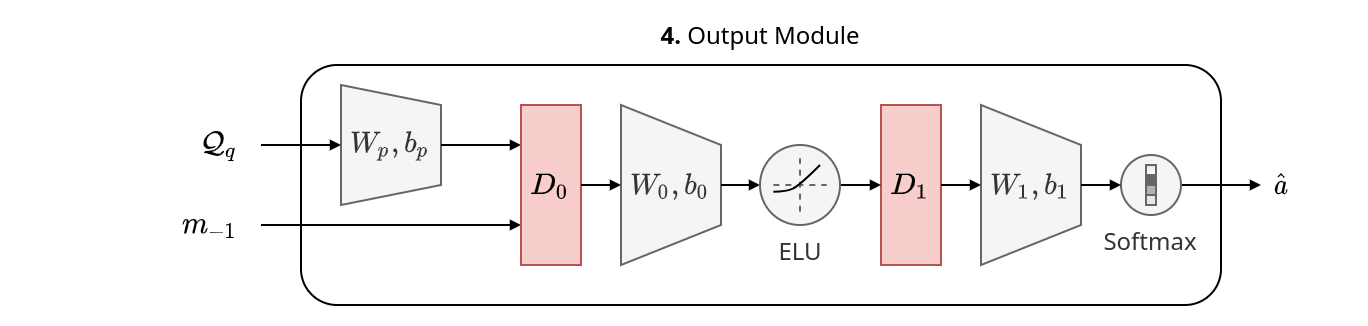
\includegraphics[width=\textwidth]{output_module.png}
    \caption{An overview of the output module, as implemented in the original paper.}
    \label{fig:output_module}
\end{figure}

{\color{red}

Move to Ablations

\begin{itemize}
  \item Concat + linear fusion (other fusion types?)
  \item Bottom-up
  \item MAC network
\end{itemize}

\subsection{Bottom-up}
\label{subsection:bottom_up}
 ReLU proved to yield higher results over gated tanh when paired with GAT/GCN embeddings. In the original paper, CNN/R-CNN features are extracted in the preprocessing step, meaning there is no need for gradient propagation to the knowledge base embedding. Preliminary tests showed a need for learnable embeddings in graph convolutional models, and thus a need for end-to-end propagation of gradients.}



\begin{itemize}
  \item Initial tests showed little performance difference between conditioning the current control state on previous control states. % #TODOInvestigate interpretability effects
\end{itemize}
